\documentclass[12pt,reqno]{amsart}
\usepackage[pdfborder={0 0 0.5 [3 2]}, plainpages=false]{hyperref}%
\usepackage[left=1in,right=1in,top=1in,bottom=1in]{geometry}%
% \usepackage[shortalphabetic]{amsrefs}%
\usepackage{amsmath}
\usepackage{enumerate}
% \usepackage{enumitem}
\usepackage{amssymb}                
\usepackage{amsmath}                
\usepackage{amsfonts}
\usepackage{amsthm}
\usepackage{bbm}
\usepackage[table,xcdraw]{xcolor}
\usepackage{tikz}
\usepackage{float}
\usepackage{booktabs}
\usepackage{svg}
\usepackage{mathtools}
\usepackage{cool}
\usepackage{url}
\usepackage{graphicx,epsfig}
\usepackage{makecell}
\usepackage{array}

\usepackage[capitalize,nameinlink]{cleveref}
% Per SIAM Style Manual, "section" should be lowercase
\crefname{section}{section}{sections}
\crefname{subsection}{subsection}{subsections}
\Crefname{section}{Section}{Sections}
\Crefname{subsection}{Subsection}{Subsections}

% Per SIAM Style Manual, "Figure" should be spelled out in references
\Crefname{figure}{Figure}{Figures}

% Per SIAM Style Manual, don't say equation in front on an equation.
\crefformat{equation}{\textup{#2(#1)#3}}
\crefrangeformat{equation}{\textup{#3(#1)#4--#5(#2)#6}}
\crefmultiformat{equation}{\textup{#2(#1)#3}}{ and \textup{#2(#1)#3}}
{, \textup{#2(#1)#3}}{, and \textup{#2(#1)#3}}
\crefrangemultiformat{equation}{\textup{#3(#1)#4--#5(#2)#6}}%
{ and \textup{#3(#1)#4--#5(#2)#6}}{, \textup{#3(#1)#4--#5(#2)#6}}{, and \textup{#3(#1)#4--#5(#2)#6}}

% But spell it out at the beginning of a sentence.
\Crefformat{equation}{#2Equation~\textup{(#1)}#3}
\Crefrangeformat{equation}{Equations~\textup{#3(#1)#4--#5(#2)#6}}
\Crefmultiformat{equation}{Equations~\textup{#2(#1)#3}}{ and \textup{#2(#1)#3}}
{, \textup{#2(#1)#3}}{, and \textup{#2(#1)#3}}
\Crefrangemultiformat{equation}{Equations~\textup{#3(#1)#4--#5(#2)#6}}%
{ and \textup{#3(#1)#4--#5(#2)#6}}{, \textup{#3(#1)#4--#5(#2)#6}}{, and \textup{#3(#1)#4--#5(#2)#6}}

% Make number non-italic in any environment.
\crefdefaultlabelformat{#2\textup{#1}#3}

\def\noi{\noindent}
\def\T{{\mathbb T}}
\def\R{{\mathbb R}}
\def\N{{\mathbb N}}
\def\C{{\mathbb C}}
\def\Z{{\mathbb Z}}
\def\P{{\mathbb P}}
\def\E{{\mathbb E}}
\def\Q{\mathbb{Q}}
\def\ind{{\mathbb I}}

\DeclareMathOperator{\spn}{span}
\DeclareMathOperator{\ran}{range}
\DeclareMathOperator{\diag}{diag}


\graphicspath{ {images/} }

\newtheorem{lemma}{Lemma}
\newtheorem{theorem}{Theorem}
\newtheorem{corollary}{Corollary}
\newtheorem{definition}{Definition}
\newtheorem{proposition}{Proposition}
\newtheorem{hypothesis}{Hypothesis}

\newtheorem{notation}{Notation}

\begin{document}

\title{Standing Wave Solutions in Twisted Multicore Fibers}

\author{Ross Parker}
\address{Department of Mathematics, Southern Methodist Univeristy, 
Dallas, TX 75275}
\email{rhparker@smu.edu}

\author{Alejando Aceves}
\address{Department of Mathematics, Southern Methodist Univeristy, 
Dallas, TX 75275}
\email{aaceves@smu.edu}

\begin{abstract}
In the present work, we consider the existence and spectral stability of standing wave solutions to a model for light propagation in a circular array of helical waveguides. Numerical parameter continuation experiments demonstrate the existence of standing wave solutions for sufficiently small values of the coupling parameter. Furthermore, standing waves exhibiting optical Aharonov-Bohm suppression, where there is a single waveguide which remains unexcited, exist when the twist parameter $\phi$ and the number of waveguides $N$ is related by $\phi = \pi/N$. Spectral computations and numerical timestepping simulations suggest that standing wave solutions where the energy is concentrated in a single site are neutrally stable. 
\end{abstract}

\maketitle

\section{Introduction}

There has been much recent theoretical and experimental interest in light dynamics in twisted multi-core optical fibers. Early work on twisted fibers can be found in \cite{Longhi2007,Longhi2007b}, in which the coupled mode equations describing light propagation in a circular arrangement of helical waveguides is derived. The introduction of a fiber twist in a circular array allows for control of diffraction and light transfer, in a similar manner to axis bending in linear waveguide arrays \cite{Longhi2005}. The fiber twist introduces additional phase terms to the model, which is known as the Peierls phase \cite{Longhi2007,Peierls1933}. This system is considered as an optical analogue of topological Aharonov-Bohm suppression of tunneling \cite{Loss1992} in \cite{Ornigotti2007}, where the fiber twist plays the role of the magnetic flux in the quantum mechanical system. Parity-time ($\mathcal{PT}$) symmetry with balanced gain and loss terms is considered in \cite{Longhi2016,castro2016}. More complicated fiber bundle geometries have since been studied, which include Lieb lattices \cite{Marzuola2019bulk} and honeycomb lattices \cite{Ablowitz2014,Lumer2013}. Experimental applications of twisted multi-core fibers include the construction of sensors for shape, strain, and temperature \cite{Gannot2014,Westbrook2017}. 

In this paper, we consider a multi-core fiber consisting of $N$ waveguides arranged in a ring (\cref{fig:ring}).
\begin{figure}[H]
\begin{center}
\includegraphics[width=4cm]{circle}
\end{center}
\caption{Schematic of $N$ twisted fibers arranged in a ring.}
\label{fig:ring}
\end{figure}
\noi Each fiber is twisted in a uniform fashion along the propagation direction $z$. For the system with an optical Kerr nonlinearity, the dynamics are given by the coupled system of equations \cite{castro2016,Parto2017}
\begin{equation}\label{eq:twist}
i \partial_z c_n = k \left(e^{-i\phi}c_{n+1} + e^{i\phi}c_{n-1}\right) + i \gamma_n c_n + d |c_n|^2 c_n 
\end{equation}
for $n = 1, \dots, N$, where $c_0 = c_{N}$ and $c_{N+1} = c_1$ due to the circular geometry. The quantities $c_n(z)$ are the complex-valued amplitudes of each waveguide, $k$ is the strength of the nearest-neighbor coupling, $\gamma_n$ is the optical gain or loss at site $n$, and $\phi$ is a parameter representing the twist of the fibers. (See \cite[section 2]{castro2016} for a description of the parameters in terms of the geometry of the optical waveguide system). If $\gamma_n = 0$ for all $n$, i.e. there is no gain or loss at each node, equation \cref{eq:twist} becomes
\begin{equation}\label{eq:twist1}
i \partial_z c_n = k \left(e^{-i\phi}c_{n+1} + e^{i\phi}c_{n-1}\right) + i \gamma_n c_n + d |c_n|^2 c_n,
\end{equation}
which is Hamiltonian with energy given by
\begin{equation}
H = \sum_{n=1}^N k (c_{n+1}c_n^* e^{-i \phi} + c_n c_{n+1}^* e^{i \phi}) + \frac{d}{2}|c_n|^4.
\end{equation}
The Hamiltonian system is considered in \cite{castro2016}, in which asymptotic analysis for $N=6$ fibers where the peak intensity is contained in the first fiber ($n=1$) is performed; most notably, the opposite fiber in the ring ($n=4$) has, to leading order, zero intensity when the twist parameter is given by $\phi = \pi/6$. This is confirmed by numerical time evolution simulations (see \cite[Figures 4 and 5]{castro2016}). This phenomenon is discussed in the context of Aharonov-Bohm (AB) suppression of optical tunneling in twisted multicore fibers in \cite{Parto2017,Parto2019}. In particular, this effect is demonstrated analytically for the case of $N = 4$ and $\phi = \pi/4$ fibers by solving the nonlinear system \cref{eq:twist} analytically. 

In this paper, we study standing wave solutions (bound states) of equation \cref{eq:twist}. This paper is organized as follows. In \cref{sec:standingwave}, we construct standing wave solutions to \cref{eq:twist}. In \cref{sec:ABsupp}, we show the existence, both analytically and numerically, of standing wave solutions which have a single dark node when $\phi = \pi/N$. We then investigate stability of these solutions in \cref{sec:stability}. We conclude with a brief discussion of asymmetric variants and some directions for future research.

\section{Standing wave solutions}\label{sec:standingwave}

Standing wave solutions to \cref{eq:twist1} are bound states of the form
\begin{equation}\label{eq:ansatz1}
c_n = a_n e^{i (\omega z + \theta_n) },
\end{equation}
where $a_n \in \R$, $\theta_n \in (-\pi/2, \pi/2]$, and $\omega$ is the frequency of oscillation. (Since we allow $a_n$ to be negative, we can restrict $\theta_n$ to that interval). Making this substitution and simplifying, equation \cref{eq:twist1} becomes
\begin{equation}\label{eq:twisteq}
k\left( a_{n+1} e^{i((\theta_{n+1}-\theta_n)-\phi)} + a_{n-1} e^{-i((\theta_n - \theta_{n-1})-\phi)}\right) + \omega a_n + d a_n^3 = 0,
\end{equation}
which can be written as the system of $2n$ equations
\begin{equation}\label{eq:twisteqreal}
\begin{aligned}
&k\left( a_{n+1} \cos(\theta_{n+1}-\theta_n-\phi) + a_{n-1} \cos(\theta_n - \theta_{n-1}-\phi)\right) + \omega a_n + d a_n^3 = 0 \\\
&a_{n+1} \sin(\theta_{n+1}-\theta_n-\phi) - a_{n-1} \sin(\theta_n - \theta_{n-1}-\phi) = 0
\end{aligned}
\end{equation}
by separating real and imaginary parts. We note that the the exponential terms in \cref{eq:twisteq} depend only on the phase differences $\theta_{n+1}-\theta_n$ between adjacent sites. Due to the gauge invariance of \cref{eq:twist1}, if $c_n$ is solution, so is $e^{i \theta} c_n$, thus we may without loss of generality take $\theta_1 = 0$. If $\phi = 0$, i.e. the fibers are not twisted, we can take $\theta_n = 0$ for all $n$, and so \cref{eq:twisteq} reduces to the untwisted case with periodic boundary conditions. Similarly, if we take $\phi = 2 \pi/N$ and $\theta_n = (n-1)\phi$ for all $n$, the exponential terms do not contribute, and \cref{eq:twisteq} once again reduces to untwisted case. The interesting case, therefore, occurs when $0 < \theta < 2 \pi/N$. 

In the anti-continuum (AC) limit, which occurs when $k = 0$, the lattice sites are decoupled. Each $a_n$ can take on the values $\{0, \pm \sqrt{-\omega/d} \}$, the phases $\theta_n$ are arbitrary, and $\phi$ does not contribute. The amplitudes $\sqrt{-\omega/d}$ are real if $d$ and $\omega$ have opposite signs. We construct solutions to \cref{eq:twisteqreal} by parameter continuation from the AC limit with no twist using AUTO. As an initial condition, we choose a single excited site at node 1, i.e. $a_1 = \sqrt{-\omega/d}$ and $a_n = 0$ for all other $n$. (We can start with more than once excited state, but, in general, these solutions will not be stable.) In addition, we take $\theta_n = 0$ for all $n$ and $\phi = 0$.  We first continue in the coupling parameter $k$, and then, for fixed $k$, we continue in the twist parameter $\phi$. In doing this, we observe that the solutions have the following symmetry:
\begin{equation}\label{eq:symm}
\begin{aligned}
a_k &= a_{N-k+2} && \qquad k = 2, \dots, M-1 \\
\theta_k &= -a_{N-k+2} && \qquad k = 2, \dots, M-1,
\end{aligned}
\end{equation}
where $M = (N/2)+1$ for $N$ even and $M = (N+1)/2$ for $N$ odd. For $N$ even, node $M$ is the node directly across the ring from node 1, and $\theta_M = 0$. For all $N$, $\theta_1 = 0$. See \cref{fig:symmetry1} for an illustration of these symmetry relations for $N = 6$ and $N = 7$. 
\begin{figure}[H]
\begin{center}
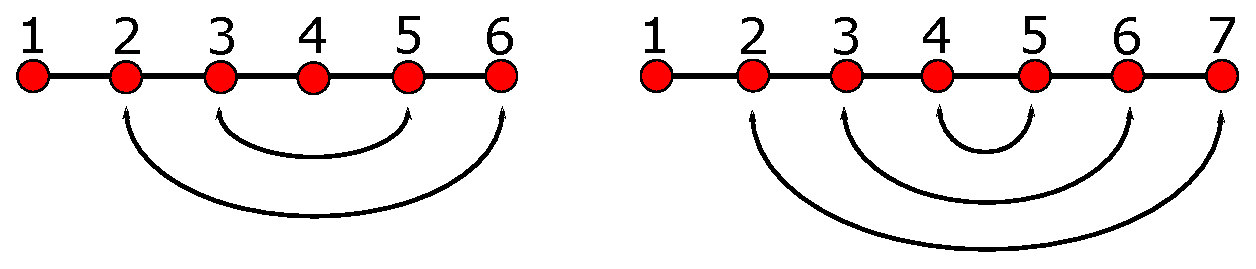
\includegraphics[width=10cm]{symmetry1.eps}
\end{center}
\caption{Schematic of symmetry relationship between nodes for $N = 6$ and $N=7$. For nodes connected with arrows, the amplitudes $a_k$ are the same and the phases $\theta_k$ are opposite.}
\label{fig:symmetry1}
\end{figure}
\noi \cref{fig:twist025} shows an example of a standing wave solution produced by numerical parameter continuation for $N = 6$. The symmetry relations \cref{eq:symm} among the amplitudes $a_k$ can be seen in the right panel.
\begin{figure}[H]
\begin{center}
\begin{tabular}{c}
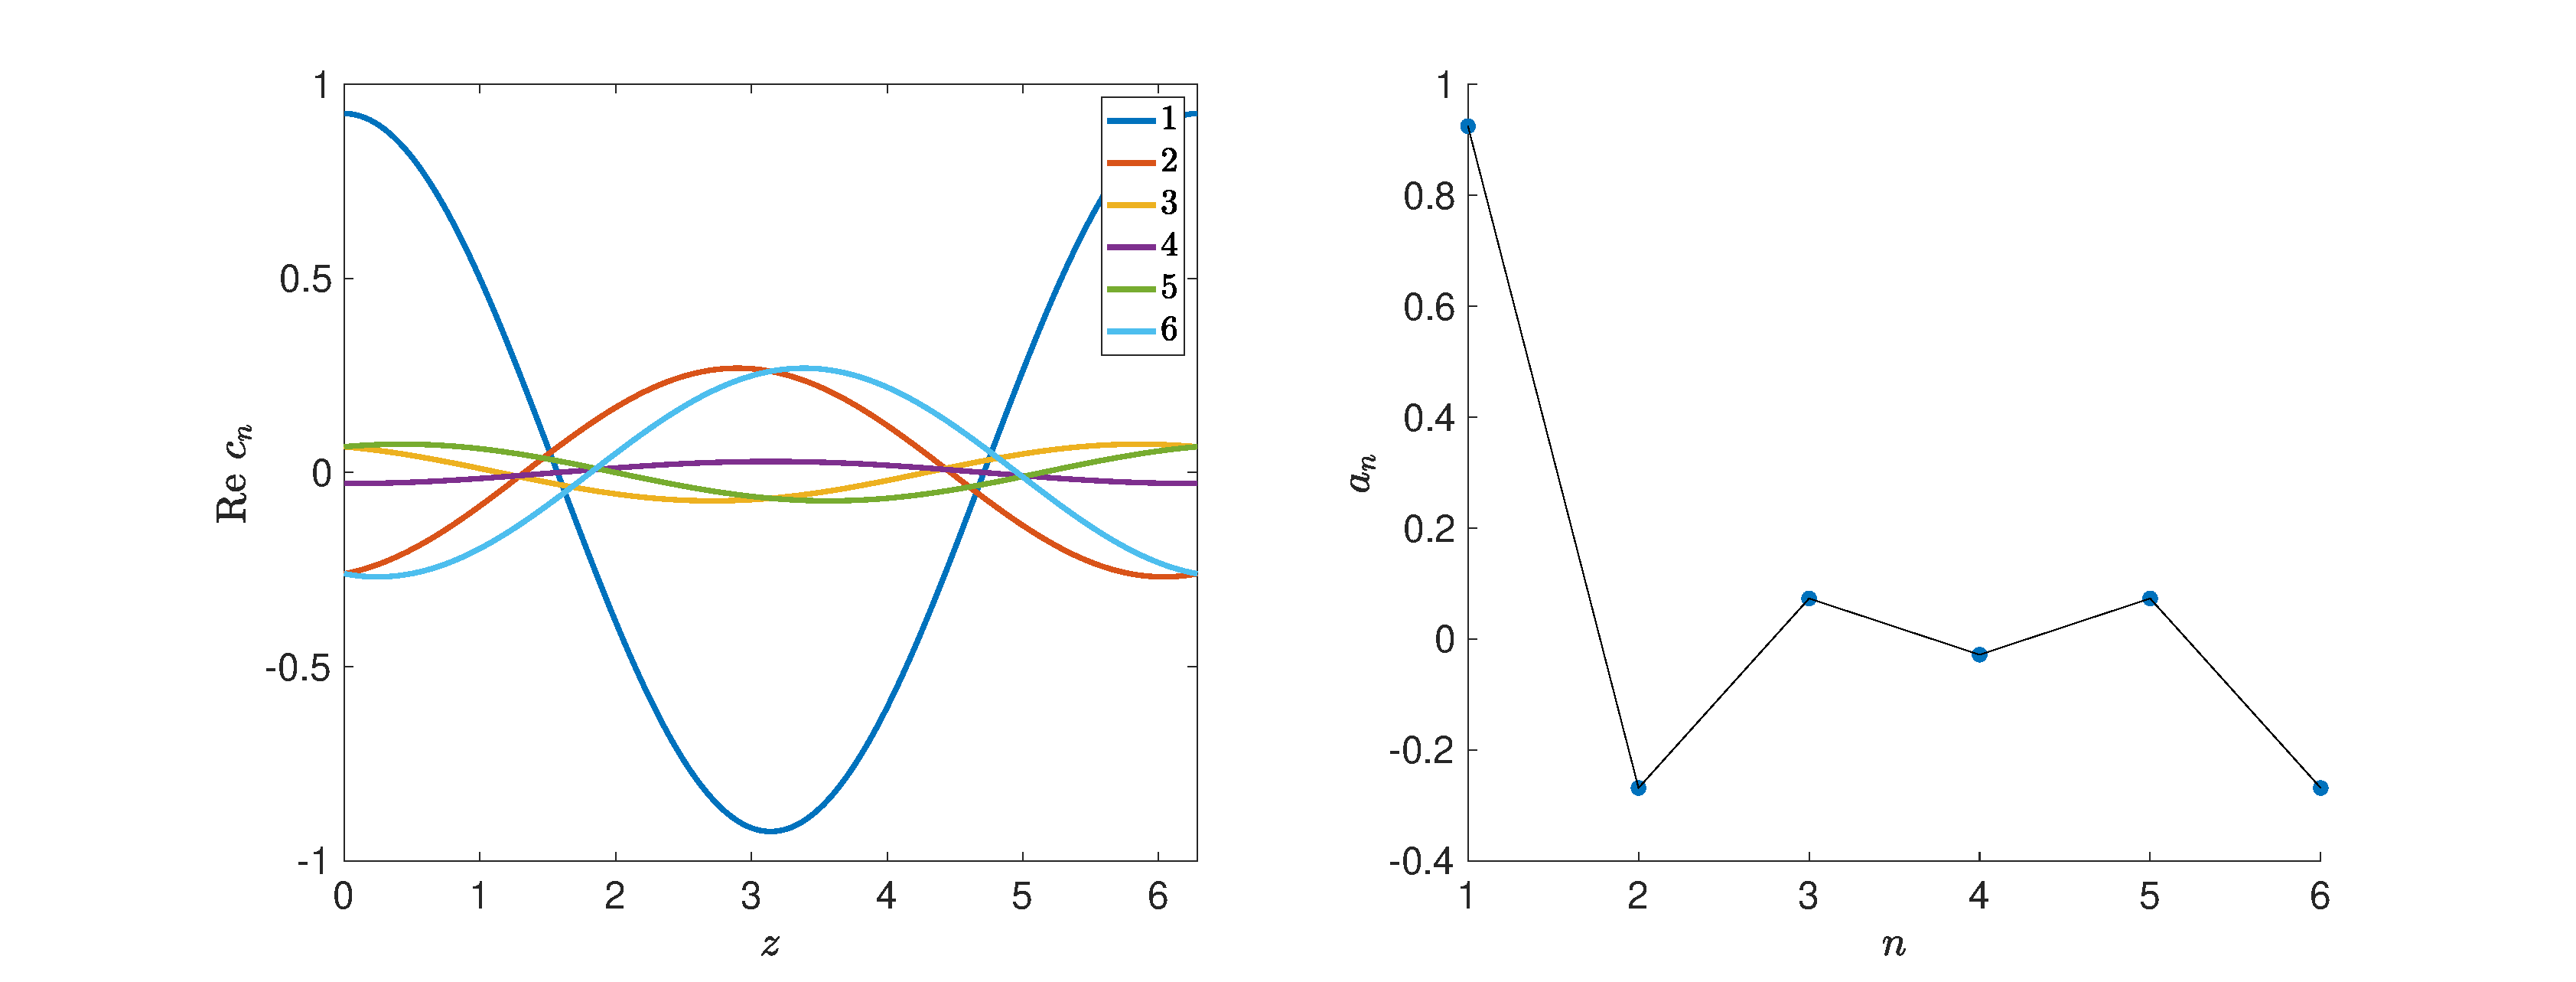
\includegraphics[width=15cm]{images/twist025.eps}
\end{tabular}
\end{center}
\caption{Standing wave solution for $N = 6$, $\omega = 1$, and $\phi = 0.25$. Left panel is real part of solution $c_n$ versus $z$ for nodes 1-4 over a full period ($2 \pi)$. The solution for the remaining nodes can be found from the symmetry relations \cref{eq:symm}. Right panel is amplitude $a_n$ solution at each node. $k = 0.25$, $d=-1$.}
\label{fig:twist025}
\end{figure}

\section{Optical Aharonov-Bohm suppression}\label{sec:ABsupp}

Numerical parameter continuation, starting from a single excited node at node 1, suggests that optical Aharonov-Bohm suppression occurs when twist parameter is $\phi = \pi/N$. For $N$ even, the node opposite node 1 in the ring is completely dark, which agrees with \cite{castro2016,Parto2017}. We now show this occurs for standing wave solutions. We consider the cases of $N$ even and $N$ odd separately, since the symmetry patterns are different. In both cases, we find that there is a single dark node when $\phi = \pi/N$.

\subsection{\texorpdfstring{$N$}{N} even}\label{sec:Neven}

Taking $a_M = 0$, where $M = (N/2)+1$, we use the symmetries the system \cref{eq:symm} to reduce the system \cref{eq:twisteqreal} to
\begin{equation}\label{eq:twisteqeven}
\begin{aligned}
&2 k a_2 \cos(\theta_2 - \phi) + \omega a_1 + d a_1^3 = 0 \\
&k( a_{n+1} \cos(\theta_{n+1}-\theta_n-\phi) + a_{n-1} \cos(\theta_n - \theta_{n-1}-\phi)) + \omega a_n + d a_n^3 = 0 && n = 2, \dots, M-1 \\
&a_{n+1} \sin(\theta_{n+1}-\theta_n-\phi) - a_{n-1} \sin(\theta_n - \theta_{n-1}-\phi) = 0 && n = 2, \dots, M-1 \\
&2 k a_{M-1} \cos(\theta_{M-1} + \phi) = 0 \\
& \theta_1 = \theta_M = 0.
\end{aligned}
\end{equation}
It follows that $a_n = 0$ for all $n$ unless
\begin{equation}\label{eq:evendarknodecond}
\begin{aligned}
&\cos(\theta_{M-1} + \phi) = 0 \\
&\sin(\theta_{n} - \theta_{n-1} - \phi) = 0 && \qquad n = 3, \dots, M-1 \\
&\sin(\theta_2 - \phi) = 0.
\end{aligned}
\end{equation}
One solution to this is
\begin{equation}\label{eq:evendarknodecond1}
\begin{aligned}
&\theta_{M-1} + \phi = \pi/2 \\
&\theta_{n} - \theta_{n-1} - \phi = 0 && n = 3, \dots, M-1 \\
&\theta_2 - \phi = 0,
\end{aligned}
\end{equation}
from which it follows that we can have a single dark node at site $M$ when $\phi = \pi/N$. If this is the case, the system of equations \cref{eq:twisteqeven} reduces to the simpler system 
\begin{equation}\label{eq:twisteqevenhole}
\begin{aligned}
&2 k a_2 + \omega a_1 + d a_1^3 = 0 \\
&k\left( a_{n+1} + a_{n-1} \right) + \omega a_n + d a_n^3 = 0 && \qquad n = 2, \dots, M-2 \\
&k a_{M-2} + \omega a_{M-1} + d a_{M-1}^3 = 0.
\end{aligned}
\end{equation}
This system is of the form $F(a,k) = 0$, where $a = (a_1, \dots, a_{M-1})$. $F(\tilde{a}, 0) = 0$, where $\tilde{a} = (\sqrt{-\omega/d}, 0, \dots, 0)$. Since $D_F(\tilde{a}, 0) = \diag(-2\omega,\omega, \dots, \omega)$, which is invertible for $\omega \neq 0$, the system \cref{eq:twisteqevenhole} has a solution for sufficiently small $k$ by the implicit function theorem. Once \cref{eq:twisteqevenhole} has been solved, the full solution to \cref{eq:twisteqreal} is given by
\begin{align*}
&a_M = 0 \\
&a_{M+k} = a_{M-k} && \qquad k = 1, \dots, M-2 \\
&\theta_0 = 0 \\
&\theta_k = (k-1)\phi && \qquad  k = 2, \dots, M-1 \\
&\theta_M = 0 \\
&\theta_{M+k} = -\theta_{M-k} && \qquad k = 1, \dots, M-2.
\end{align*}
\cref{fig:evenhole6} shows this solution for $N=6$. This observation of a dark node for $N = 6$ when $\phi = \pi/6$ agrees with what was shown in \cite{castro2016}. 
\begin{figure}[H]
\begin{center}
\begin{tabular}{c}
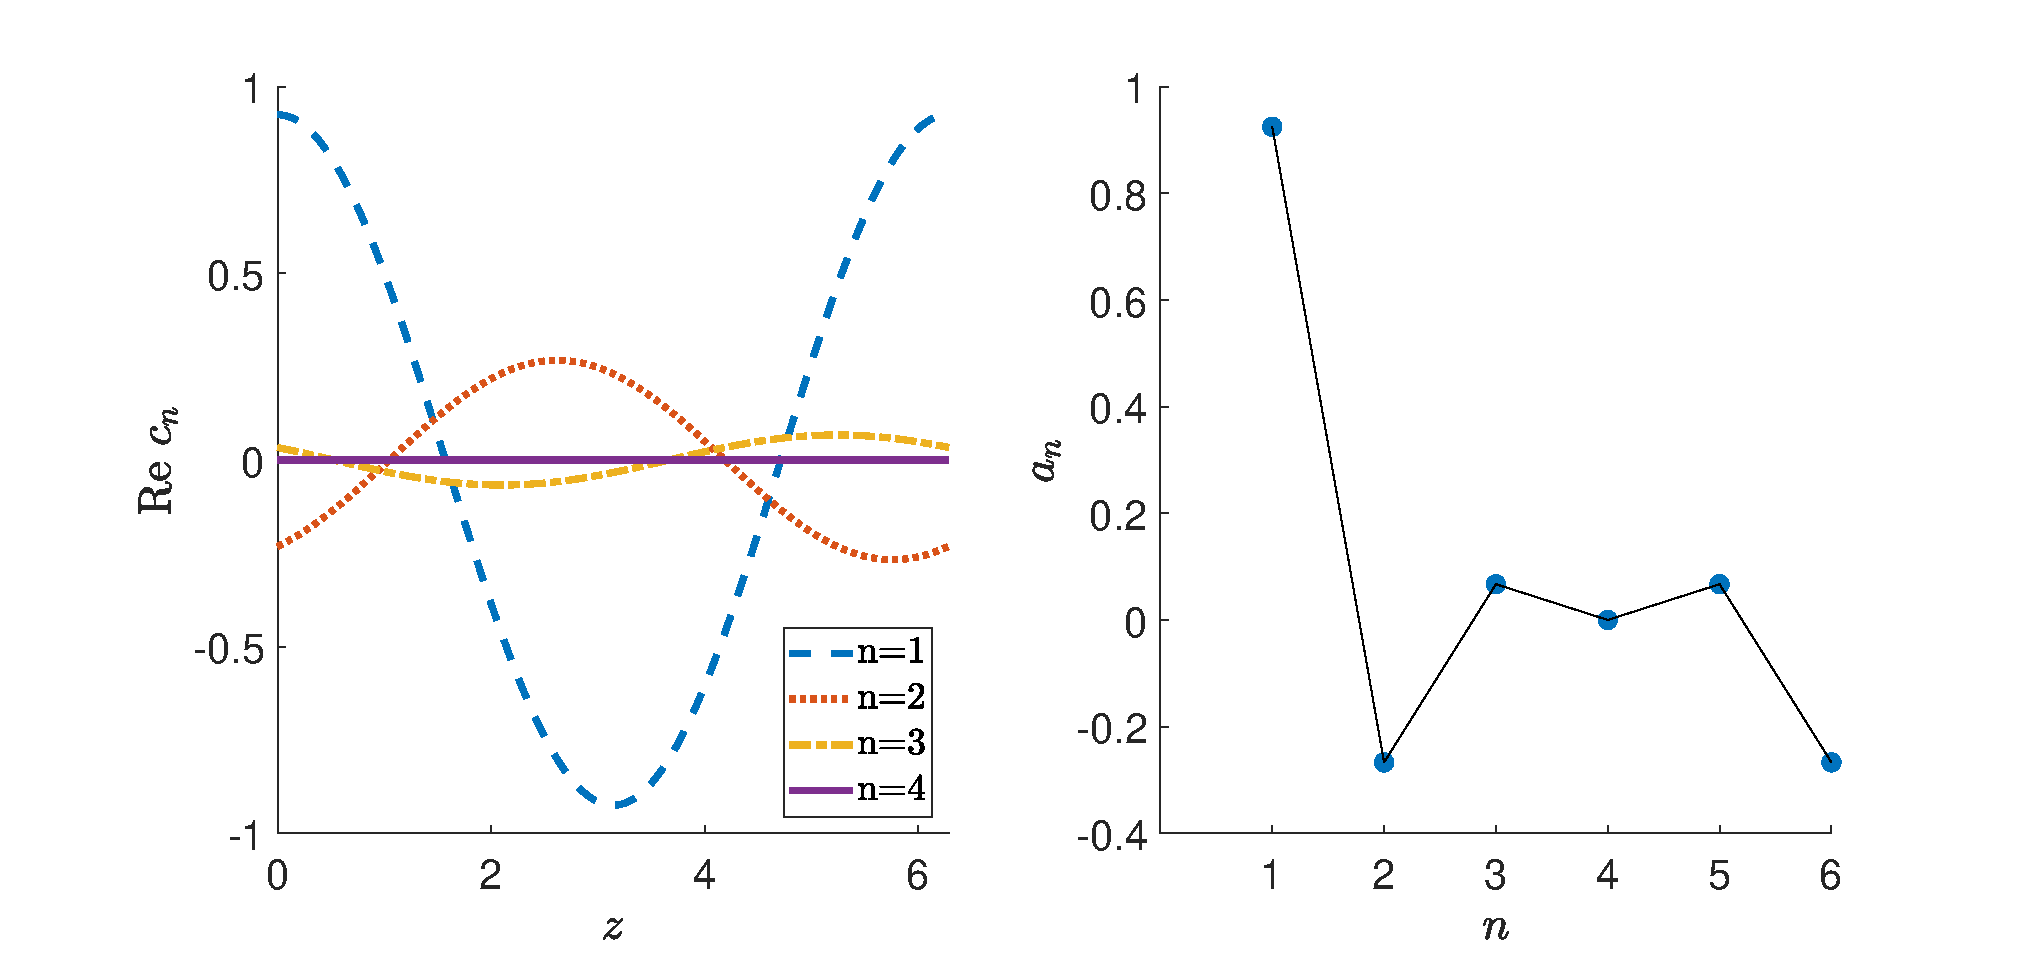
\includegraphics[width=15cm]{images/evenhole6.eps}
\end{tabular}
\end{center}
\caption{Standing wave solution for $N = 6$ and $\phi = \pi/6$. Left panel is real part of solution for nodes 1-4, right panel is absolute value of solution at each node. Node 1 has maximum amplitude, and node 4 is a dark node. $\omega = 1$, $k = 0.25$, $d=-1$.}
\label{fig:evenhole6}
\end{figure}
Numerical parameter continuation with AUTO shows that these standing wave solutions exist for $|k| \leq k_0$, where $k_0$ depends on $N$ and $\omega$ but not $d$ (\cref{fig:evenbif}, left panel). The dependence of $k_0$ on $\omega$ is shown in the right panel of \cref{fig:evenbif}, which suggests that $k_0$ approaches $\omega/2$ as $N$ gets large. As $k$ approaches $k_0$ in the parameter continuation, the solution approaches the zero solution. 
\begin{figure}[H]
\begin{center}
\begin{tabular}{cc}
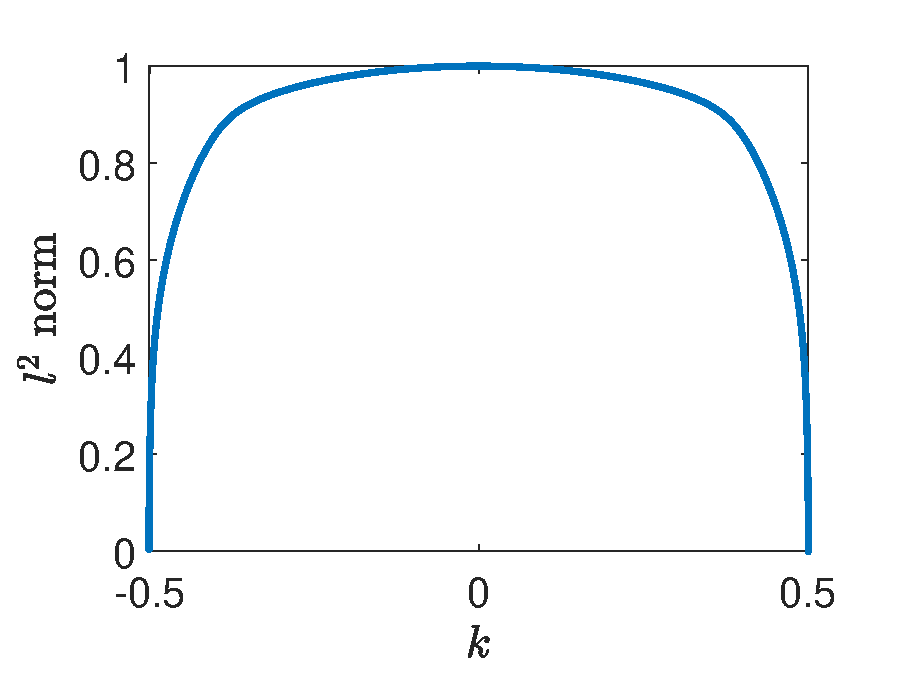
\includegraphics[width=8cm]{evenbif50.eps} &
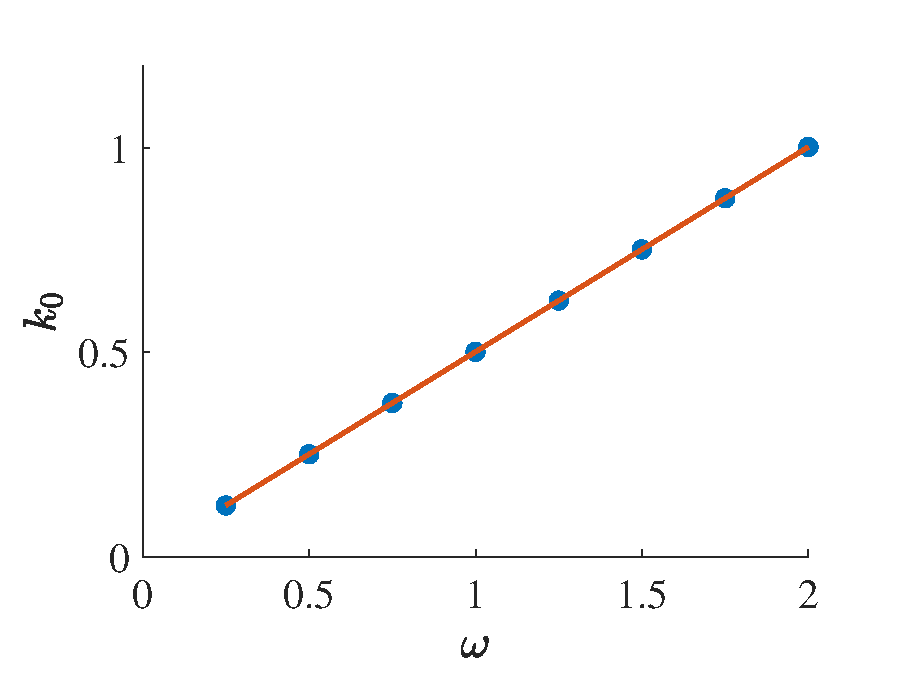
\includegraphics[width=8cm]{k0vsomega.eps}
\end{tabular}
\end{center}
\caption{Left panel shows $l^2$ norm of solution vs $k$, for $N = 50$ with dark node at node 4, $\omega = 1$, and $d=-1$. Right panel shows $k_0$ vs $\omega$ together with least squares linear regression line for $N = 50$ and $d = -1$.}
\label{fig:evenbif}
\end{figure}

\subsection{\texorpdfstring{$N$}{N} odd}\label{sec:Nodd}

We can also obtain a dark node when $N$ is odd. For simplicity, we take node 1 to be the dark node; in this case, the dark node will be opposite a pair of bright nodes at $a_M$ and $a_{M+1}$ with the same amplitude, where $M = (N+1)/2$. Using the symmetries \cref{eq:symm}, when $a_1 = 0$, the system \cref{eq:twisteqreal} reduces to 
\begin{equation}\label{eq:twisteqodd}
\begin{aligned}
&2 k a_2 \cos(\theta_2 - \phi) = 0 \\
&k a_3 \cos(\theta_3-\theta_2-\phi) + \omega a_2 + d a_2^3 = 0 \\
&a_3 \sin(\theta_3-\theta_2-\phi) = 0 \\
&k\left( a_{n+1} \cos(\theta_{n+1}-\theta_n-\phi) + a_{n-1} \cos(\theta_n - \theta_{n-1}-\phi)\right) + \omega a_n + d a_n^3 = 0 && n = 3, \dots, M-1 \\
&a_{n+1} \sin(\theta_{n+1}-\theta_n-\phi) - a_{n-1} \sin(\theta_n - \theta_{n-1}-\phi) = 0 && n = 3, \dots, M-1 \\
&k ( a_M \cos(-2 \theta_M - \phi) + a_{M-1} \cos(\theta_M - \theta_{M-1} - \phi)) + \omega a_M + d a_M^3 = 0 \\
& a_M \sin(-2 \theta_M - \phi) - a_{M-1} \sin(\theta_M - \theta_{M-1} - \phi) = 0.
\end{aligned}
\end{equation}
It follows that $a_n = 0$ for all $n$ unless
\begin{equation}\label{eq:odddarknodecond}
\begin{aligned}
&\cos(\theta_2 - \phi) = 0 \\
&\sin(\theta_{n} - \theta_{n-1} - \phi) = 0 && \qquad n = 3, \dots, M-1 \\
&\sin(2 \theta_M + \phi) = 0.
\end{aligned}
\end{equation}
One solution to this is
\begin{equation}\label{eq:odddarknodecond1}
\begin{aligned}
&\theta_2 - \phi = -\pi/2 \\
&\theta_{n} - \theta_{n-1} - \phi = 0 && \qquad n = 3, \dots, M-1 \\
&2 \theta_M + \phi = 0,
\end{aligned}
\end{equation}
from which it follows that we can have a single dark node at $a_1$ when $\phi = \pi/N$. This condition for a dark node is the same as for the $N$ even case. For this case, \cref{eq:twisteqodd} reduces to the simpler system of equations
\begin{equation}\label{eq:twisteqoddhole}
\begin{aligned}
& k a_3 + \omega a_2 + d a_2^3 = 0\\
&k( a_{n+1} + a_{n-1} ) + \omega a_n + d a_n^3 = 0 && \qquad n = 3, \dots, M-1 \\
&k ( a_M + a_{M-1} ) + \omega a_M + d a_M^3 = 0.
\end{aligned}
\end{equation}
This system of equations is again of the form $F(a,k) = 0$, where $a = (a_2, \dots, a_M)$. $F(\tilde{a}, 0) = 0$, where $\tilde{a} = (0, \dots, 0, \sqrt{-\omega/d}, 0)$. Since $D_F(\tilde{a}, 0) = \diag(\omega, \dots, \omega, -2\omega)$, which is invertible for $\omega \neq 0$, the system \cref{eq:twisteqoddhole} has a solution for sufficiently small $k$ by the implicit function theorem. Once \cref{eq:twisteqoddhole} has been solved, we obtain the full solution to \cref{eq:twisteqreal} using
\begin{align*}
&a_1 = 0 \\
&a_{M+k} = a_{M-k+1} && \qquad k = 1, \dots, M-1 \\
&\theta_0 = 0 \\
&\theta_k = (k-1)\phi - \pi/2 && \qquad k = 2, \dots, M \\
&\theta_{M+k} = -\theta_{M-k+1} && \qquad k = 1, \dots, M-1
\end{align*}
\cref{fig:oddhole7} shows this solution for $N=7$. The results of parameter continuation simulations are similar to that of the $N$ even case.
\begin{figure}[H]
\begin{center}
\begin{tabular}{c}
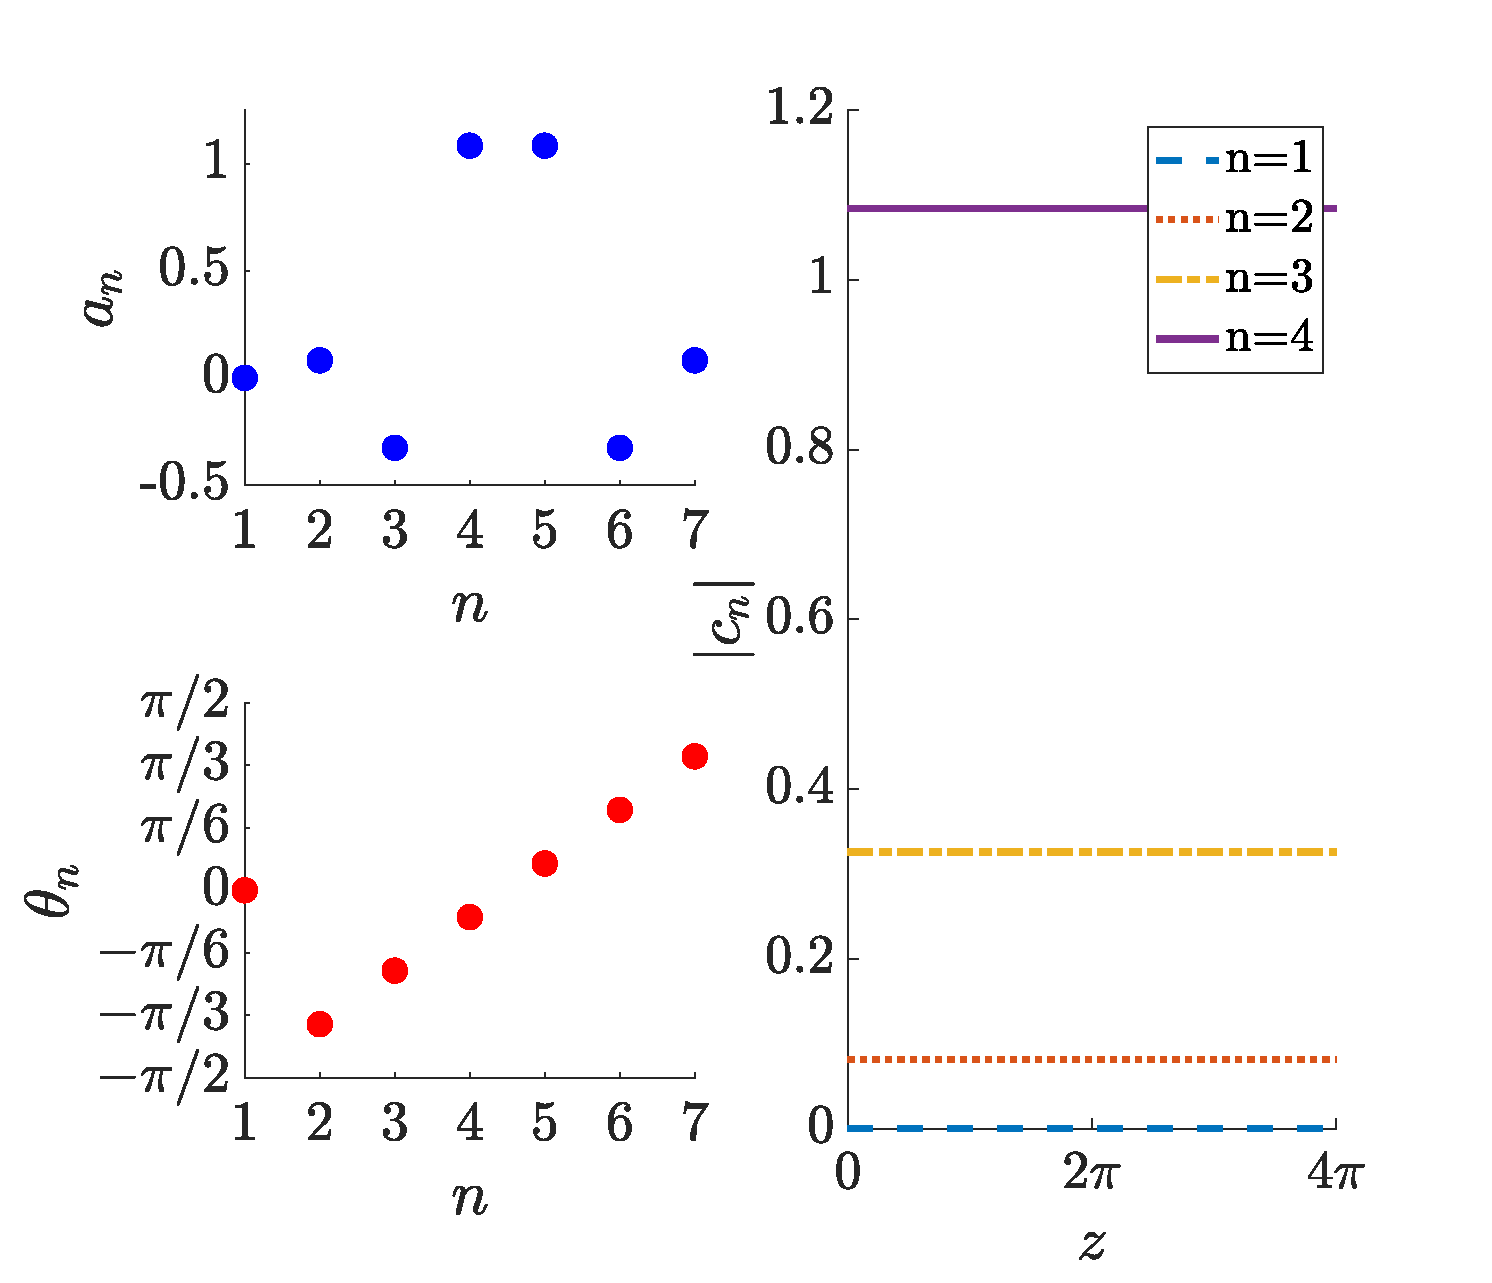
\includegraphics[width=15cm]{images/oddhole7.eps}
\end{tabular}
\end{center}
\caption{Standing wave solution for $N = 7$ and $\phi = \pi/7$. Left panel is real part of solution for nodes 1-4, right panel is absolute value of solution at each node. Nodes 4 and 5 have equal and maximum amplitude, and node 1 is a dark node. $\omega = 1$, $k = 0.25$, $d=-1$.}
\label{fig:oddhole7}
\end{figure}

\section{Stability}\label{sec:stability}

We now look at the stability of the standing wave solutions we constructed in the previous section. The linearization of equation \cref{eq:twist1} about a standing wave solution $c_n = a_n e^{i (\omega z + \theta_n) } = (v_n + i w_n)e^{i\omega z}$ is the $2N \times 2N$ block matrix
\begin{align}\label{eq:linearization}
A(c_n) =
k \begin{pmatrix}S & C \\ -C & S \end{pmatrix}
+ \omega\begin{pmatrix}0 & I \\ -I & 0 \end{pmatrix} 
+ \begin{pmatrix} \diag(2v_n w_n) & \diag(v_n^2 + 3 w_n^2) \\
-\diag(3 v_n^2 + w_n^2) & -\diag(2v_n w_n) \end{pmatrix}
\end{align}
where each block is a $N\times N$ matrix, $C$ is the periodic banded matrix with $\cos \phi$ on the first upper and lower diagonals, and $S$ is the periodic banded matrix with $\sin \phi$ on the first lower diagonal and $-\sin \phi$ on the first upper diagonal, i.e.
\begin{align*}
C &= \begin{pmatrix}
0 & \cos \phi & & \dots & \cos \phi \\
\cos \phi & 0 & \cos \phi & & & \\
& & \ddots & \ddots &  & \\
\cos \phi & & \dots & \cos \phi & 0
\end{pmatrix} \\
S &= \begin{pmatrix}
0 & -\sin \phi & & \dots & \sin \phi \\
\sin \phi & 0 & -\sin \phi & & & \\
& & \ddots & \ddots &  & \\
-\sin \phi & & \dots & \sin \phi & 0
\end{pmatrix}.
\end{align*}
Since \cref{eq:linearization} is a finite dimensional matrix, the spectrum is purely point spectrum. Due to the gauge invariance, there an eigenvalue at 0 with algebraic multiplicity 2 and geometric multiplicity 1. Following the analysis in \cite[Section 2.1.1.1]{Kevrekidis2009}, there are plane wave eigenfunctions which are, to leading order, of the form $e^{\pm( i q n + \lambda z)}$ and satisfy the dispersion relation
\begin{equation}\label{eq:dispersion}
\lambda = \pm i \left( \omega + 2 k \cos(q + \phi) \right).
\end{equation}
The corresponding eigenvalues are thus purely imaginary and are contained in the bounded intervals $\pm i[\omega - 2 k, \omega + 2 k]$. As $N$ increases, these eigenvalues fill out this interval. For $|k| < k_0 = \omega/2$, these eigenvalues cannot interact with the kernel eigenvalues. \cref{fig:evenholespec} illustrates these results numerically for $\omega = 1$ and $k = 0.25$ for the case of $N$ even $\phi = \pi/N$, i.e. a single dark node opposite a single bright node. Similar results are obtained for other values of $\omega$ and $k$ with a single bright node as well as the solutions from Section \ref{sec:Nodd}.
\begin{figure}[H]
\begin{center}
\begin{tabular}{cc}
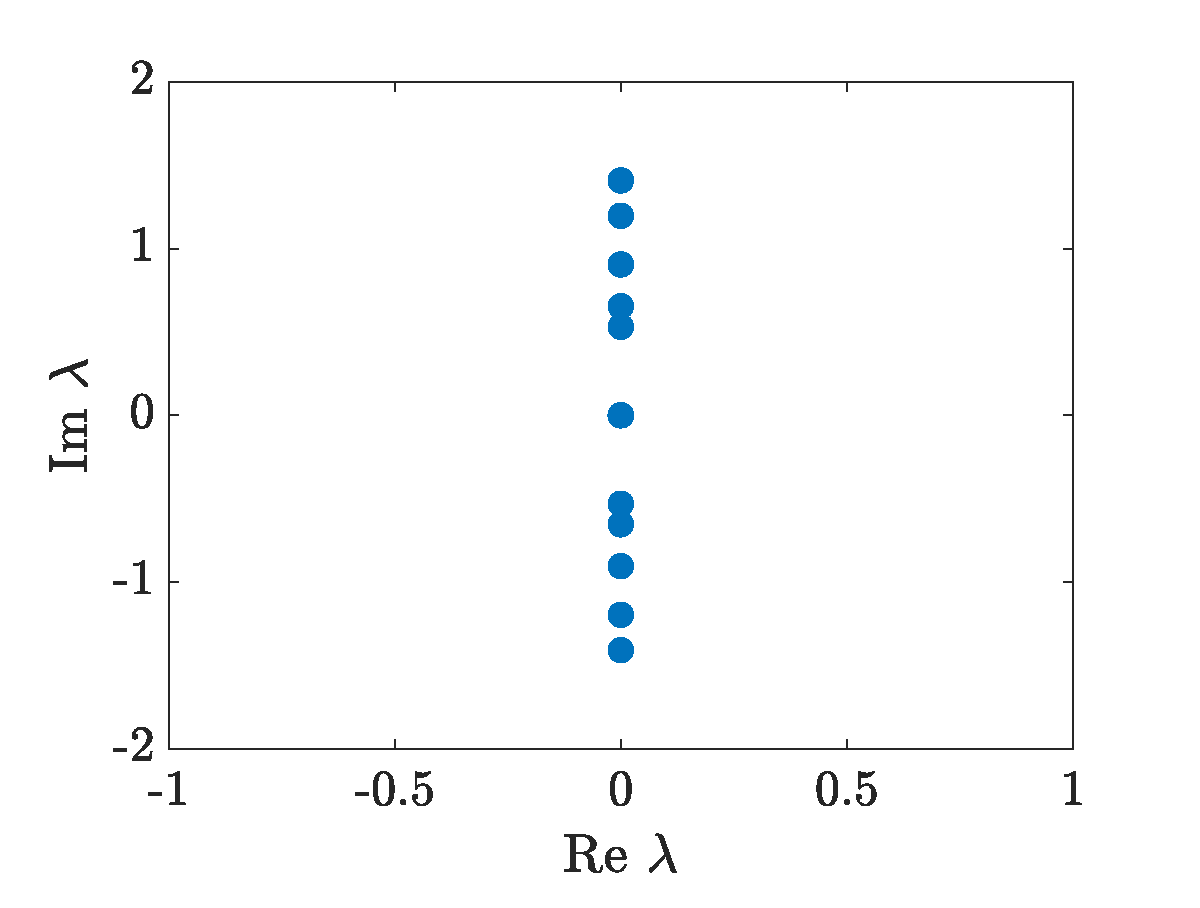
\includegraphics[width=8cm]{images/evenhole6spec.eps}
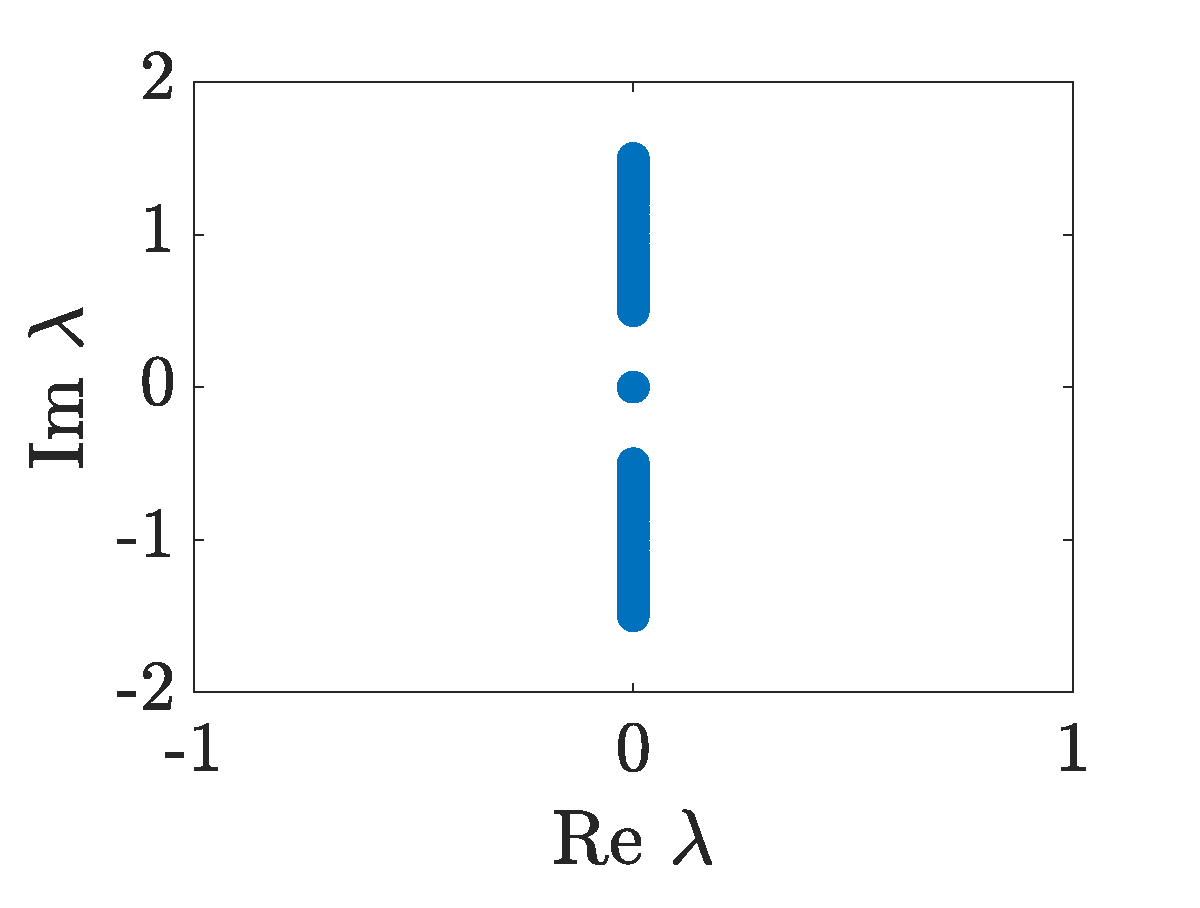
\includegraphics[width=8cm]{images/evenhole50spec.eps}
\end{tabular}
\end{center}
\caption{Spectrum of linearization of \cref{eq:twist1} about solution for even $N$ with a single dark node opposite a single bright node. $N=6$ (left panel) and $N=50$ (left panel). $k=0.25$, $\omega = 1$, $\phi = \pi/N$.}
\label{fig:evenholespec}
\end{figure}

Since the spectrum of these solutions is purely imaginary, we expect that they will be neutrally stable.  \cref{fig:evenhole6perturbed} shows the results of timestepping for a small perturbation of the standing wave solution when $N=6$. The solutions show small oscillations but no growth, which provides evidence for neutral stability. Similar results are obtained for other values of $N$ and $\omega$. In addition, if we start with a neutrally stable standing wave solution and perturb the system by a small change in $k$ or $\phi$, the time evolution resembles that in \cref{fig:evenhole6perturbed}.
\begin{figure}[H]
\begin{center}
\begin{tabular}{cc}
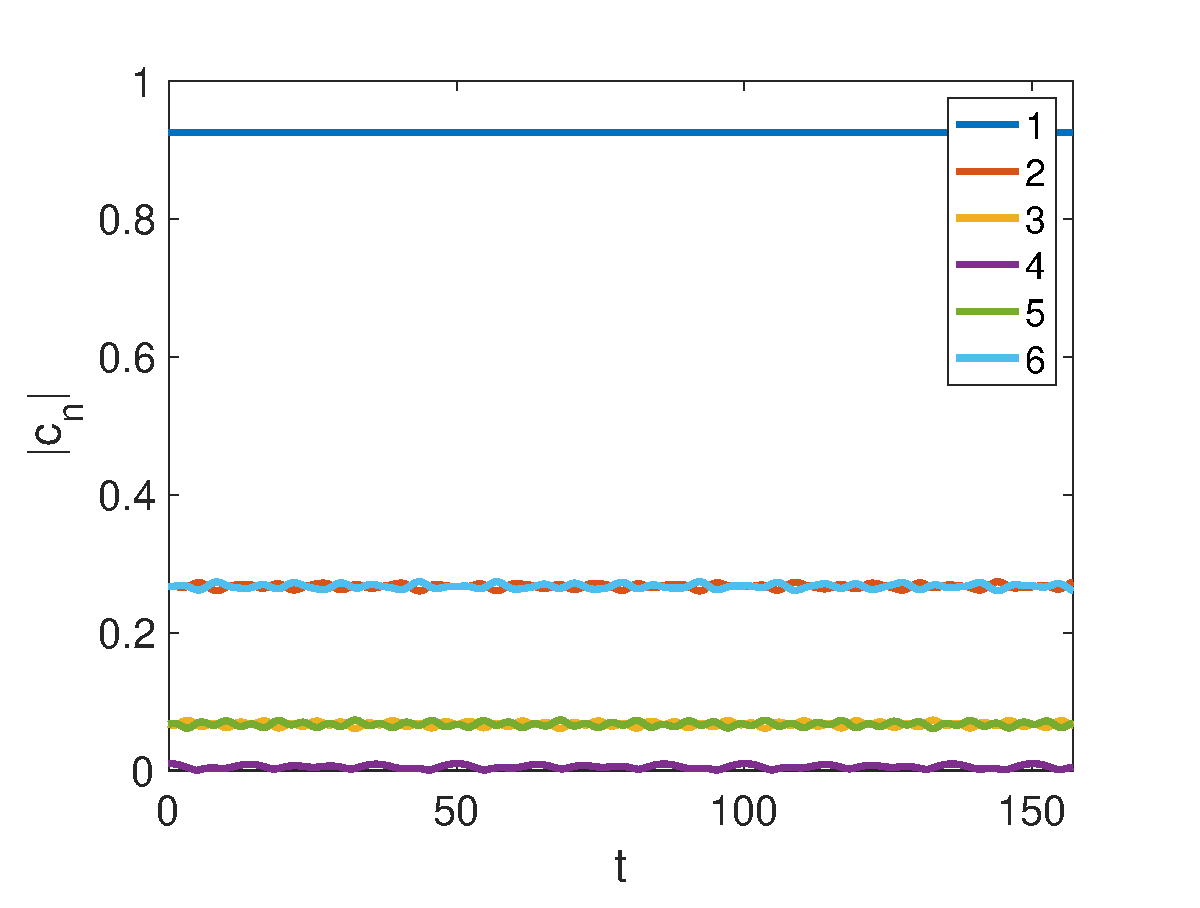
\includegraphics[width=8cm]{images/evenhole6perturbed.eps} & 
\includegraphics[width=8cm]{images/oddhole7perturbed.eps
\end{tabular}
\end{center}
\caption{Amplitude $|c_n|$ for first four nodes versus $z$ for solution with $N=6$ and $\phi = \pi/6$ (left panel) and $N=7$ and $\phi = \pi/7$ (right panel). Initial condition is perturbed by adding 0.01 to dark node. Timestepping using a fourth order Runge-Kutta scheme. $k=0.25$, $d=-1$, $\phi=\pi/6$.}
\label{fig:evenhole6perturbed}
\end{figure}

\section{Variants}\label{sec:variants}

If the strength of the nearest-neighbor coupling is allowed to differ between pairs of nodes, equation \cref{eq:twist1} becomes
\begin{equation}\label{eq:twistk}
i \partial_z c_n = k_{n+1} e^{-i\phi}c_{n+1} + k_{n-1} e^{i\phi}c_{n-1} + i \gamma_n c_n + d |c_n|^2 c_n.
\end{equation}
This allows for asymmetric solutions, as shown in \cref{fig:even6assym}. (Contrast to the symmetric solutions for uniform $k$ in \cref{fig:twist025}). These asymmetric solutions are also neutrally stable. 

\begin{figure}[H]
\begin{center}
\begin{tabular}{c}
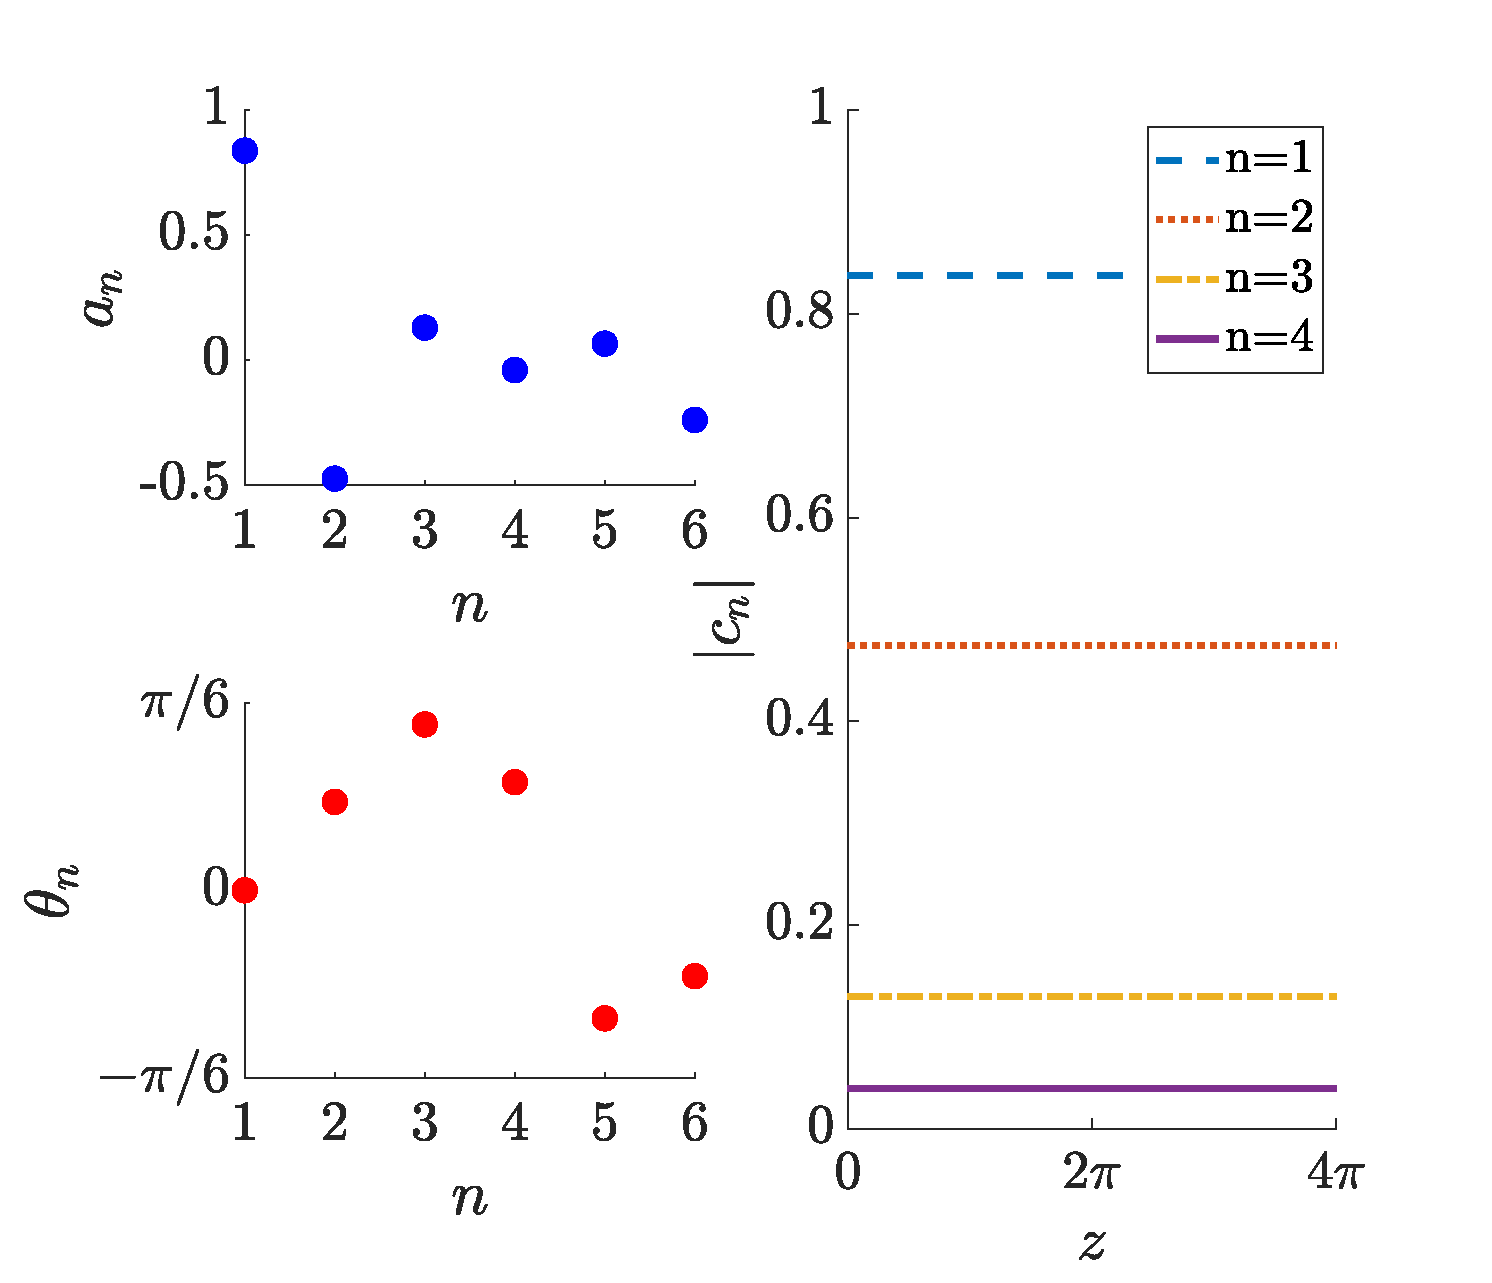
\includegraphics[width=15cm]{images/even6assym.eps}
\end{tabular}
\end{center}
\caption{Standing wave solution to \cref{eq:twistk} for $N = 6$. $\omega = 1$, $k_1 = 0.4$, and $k_n = 0.2$ for all other $n$. Left is real part of solution $c_n$ versus $z$ for nodes 1-4 over a full period ($2 \pi)$, right is amplitude $a_n$ solution at each node. $\phi = 0.25$, $d=-1$.}
\label{fig:even6assym}
\end{figure}

\section{Conclusions}

In this paper, we have demonstrated the existence of standing wave solutions to a system of equations modeling light propagation in a twisted multi-core fiber in the setting of no gain or loss at the individual sites. If the twist parameter $\phi$ and the number of waveguides $N$ are related by $\phi = \pi/N$, then standing wave solutions exist which exhibit optical Aharonov-Bohm suppression, i.e. there is a node which is completely dark for all time. These solutions exist for both $N$ even and $N$ odd, and are all neutrally stable. For future research, it would be interesting to investigate whether such standing waves exist for twisted optical fibers in more complicated geometries such as multiple concentric rings or Lieb lattices. We could also investigate the existence and stability of breather solutions, which are localized, periodic structures that are not standing waves. (See \cite{Lumer2013} for examples of breather solutions in honeycomb lattices). Finally, we could apply the techniques used here to the $\mathcal{PT}$-symmetric system with symmetric gain and loss, which is studied in \cite{castro2016}.

\section*{Acknowledgments}

This material is based upon work supported by the U.S. National Science Foundation under the RTG grant DMS-1840260 (R.P. and A.A.). The authors would also like to thank P.G. Kevrekidis for his helpful comments and suggestions for numerical simulations.

\bibliographystyle{amsplain}
\bibliography{twist.bib}


\end{document}